% !TeX program = pdflatex
% =============================================================================
% Arbeitsblatt 2: Gewitter und Faradayscher Kaefig
% UZH Praktikum I -- Sara Romer Urban, Kantonsschule im Lee, HS2026
% Klasse: 1f (09.09.2026), aus PLAN_Dokumentengenerierung.md.
%
% Direkte Fortsetzung von arbeitsblatt1-ladung-e-feld.tex (02.09.2026).
% Deckt Gewitter/Faradayscher Kaefig/Schrittspannung ab (LZ1-4), siehe
% e-feld-vertiefung-lektionsplan.tex fuer die Planungsgrundlage/Zeitbudget.
% Der Stromkreis-Teil (urspruenglich LZ5-9, Wasserkreislauf-Analogie und
% Gruppenpuzzle zu Strom/Spannung/Widerstand) wurde auf Wunsch nach
% arbeitsblaetter/elektrizitaet/u-i-r/ verschoben, da er inhaltlich zu jener
% Doppellektion (16.09.2026) gehoert -- siehe dort gruppenpuzzle3-u-i-r.tex.
% lernziele.md deckt entsprechend nur noch LZ1-4 ab; die Arbeitshypothese
% aus deren Kopfabschnitt (eine gemeinsame Doppellektion) ist damit
% zugunsten der Trennung entschieden.
%
% Kein Aufgabenblatt zu diesem Thema: laut institutionen/UZH-Praktikum-I/
% CLAUDE.md ist ein Aufgabenblatt fuer Aufgaben reserviert, die eine
% PhET-Simulation oder eine Excel-Vorlage brauchen -- fuer dieses Thema ist
% laut lernziele.md/Lektionsplan keine von beidem vorgesehen (reines
% Papier-/Demo-/Gruppenarbeits-Material), analog zu arbeitsblatt1-ladung-e-feld
% (ebenfalls ohne Aufgabenblatt).
%
% Elektroskop.svg und die fuenf Faraday_*.png sind KEINE Fotos eines realen
% Aufbaus, sondern gezeichnete Diagramme. Elektroskop.svg zeigt nur den
% Aufbau eines Elektroskops (dient als Verstaendnishilfe vor dem Experiment).
% Faraday_0.png zeigt den Kaefig/Elektroskop-Aufbau ohne Feldlinien und dient
% als Vorlage, auf der die SuS ihre eigene Skizze vervollstaendigen.
% Faraday_1.png-Faraday_4.png zeigen dagegen bereits das fertige Ergebnis
% dieser Skizze (LZ2, Ladungsverteilung/Influenz/Feld im Kaefig) und werden
% deshalb absichtlich erst in der Loesung verwendet (Konvention "SuS selbst
% ergaenzen lassen", CLAUDE.md).
% Tesla_Spule.JPG (urspruenglich in lernziele.md unter "Nicht verwendete
% Bilder" eingeplant) wird inzwischen doch verwendet, als eindruecklicher
% Grossmassstab-Aufhaenger direkt vor dem Elektroskop-Experiment.
% Nicht verwendet: electric-field-compensation-static.svg (allgemeine
% Platten-Variante derselben Physik wie die Faraday-Bildfolge -- redundant).
% =============================================================================
\documentclass[addpoints,11pt,a4paper]{exam}

\usepackage[T1]{fontenc}
\usepackage[utf8]{inputenc}
\usepackage[ngerman]{babel}
\usepackage{lmodern}
\usepackage[a4paper,margin=2.2cm,headheight=14pt]{geometry}
\usepackage{amsmath}
\usepackage{siunitx}
% Hausstil: zusammengesetzte Einheiten immer als echter Bruch (\frac), nicht
% als Inline-Schraegstrich oder \tfrac -- gilt global fuer jedes \si/\SI.
\sisetup{per-mode=fraction,fraction-command=\frac}
\usepackage{array,booktabs,tabularx,multirow}
\usepackage{enumitem}
\usepackage{xcolor}
\usepackage{colortbl}
\usepackage{tikz}
\usepackage{physics}
\usepackage[most]{tcolorbox}
\usepackage{lastpage}
\usepackage{graphicx}
\usepackage{hyperref}

\usetikzlibrary{arrows.meta,calc,angles,quotes}

% "Faraday" ist ein Eigenname und daher fuer die ngerman-Trennmuster
% unbekannt -- ohne diesen Hinweis kann "Faradayscher"/"Faradayschen" nicht
% getrennt werden, was an einer Stelle zu einer Overfull \hbox fuehrt.
\hyphenation{Fa-ra-day-scher Fa-ra-day-schen}

\usepackage{setspace}
\usepackage{needspace}
\setlength{\parindent}{0pt}
\setlength{\parskip}{0.6em}
\setstretch{1.08}
\setlist[itemize]{itemsep=0.4em}

% -----------------------------
% Farben (Corporate-Farbschema Physik KFR)
% -----------------------------
\definecolor{titleblue}{HTML}{183A6B}
\definecolor{accentblue}{HTML}{2E6F9E}
\definecolor{lightblue}{HTML}{EAF4FB}
\definecolor{lightgray}{HTML}{F4F6F8}
\definecolor{darkgray}{HTML}{4A4A4A}
\definecolor{accentorange}{HTML}{D9720C}
\definecolor{accentpurple}{HTML}{7B2D8E}
\definecolor{lightorange}{HTML}{FCEEE0}
\definecolor{lightpurple}{HTML}{F3EAF7}

% Links (hyperref): farblich ans Corporate-Farbschema angeglichen.
\hypersetup{
  colorlinks=true,
  urlcolor=accentblue,
  linkcolor=accentblue,
  pdftitle={Arbeitsblatt 2: Gewitter und Faradayscher Kaefig},
  pdfauthor={Loris Keller}
}

% -----------------------------
% Spaltentypen
% -----------------------------
\newcolumntype{Y}{>{\centering\arraybackslash}X}
\newcolumntype{P}[1]{>{\raggedright\arraybackslash}p{#1}}

% -----------------------------
% Boxen
% -----------------------------
\tcbset{before skip=10pt, after skip=10pt}
\newtcolorbox{titlebox}{
  enhanced,
  colback=titleblue,
  colframe=titleblue,
  boxrule=0pt,
  arc=3mm,
  left=3mm,right=3mm,top=3mm,bottom=3mm
}

\newlength{\aufgabenindent}
\settowidth{\aufgabenindent}{10.\hskip\labelsep}

% Praktikum I: Lernziele/Einleitung/Theorie/Aufgaben werden NICHT farbig
% gerahmt (nur Formel-, Hinweis- und Antwortbox bleiben Boxen) -- siehe
% institutionen/UZH-Praktikum-I/CLAUDE.md, Abschnitt "Boxen-Layout".
\newenvironment{infobox}{%
  \par\addvspace{10pt}\noindent
}{%
  \par\addvspace{10pt}
}

\newenvironment{theoriebox}[1][Theorie]{%
  \par\addvspace{10pt}\noindent\textbf{#1}\par\smallskip\noindent
}{%
  \par\addvspace{10pt}
}

\newtcolorbox{taskbox}[1][]{
  enhanced, breakable,
  colback=white, colframe=white, boxrule=0pt,
  left=0mm,right=0mm,top=0mm,bottom=0mm,
  before skip=10pt, after skip=10pt,
  before upper={%
    \def\tmpboxtitle{#1}%
    \ifx\tmpboxtitle\empty\else\noindent\textbf{#1}\par\smallskip\fi
  }
}

\newtcolorbox{groupbox}[1][Gruppenarbeit]{
  enhanced, breakable,
  colback=white, colframe=white, boxrule=0pt,
  left=0mm,right=0mm,top=0mm,bottom=0mm,
  before skip=10pt, after skip=10pt,
  before upper={\noindent\textbf{#1}\par\smallskip}
}

\newenvironment{beispielbox}[1][Beispiel]{%
  \par\addvspace{10pt}\noindent\textbf{#1}\par\smallskip\noindent
}{%
  \par\addvspace{10pt}
}

\newtcolorbox{hinweisbox}[1][Hinweis]{
  enhanced,
  breakable,
  colback=lightorange,
  colframe=accentorange,
  title={#1},
  fonttitle=\bfseries,
  boxrule=0.7pt,
  arc=2mm,
  left=5mm,right=5mm,top=2mm,bottom=2mm
}

\newtcolorbox{formelbox}[1][Formel]{
  enhanced,
  breakable,
  colback=lightpurple,
  colframe=accentpurple,
  title={#1},
  fonttitle=\bfseries,
  boxrule=0.9pt,
  arc=2mm,
  left=5mm,right=5mm,top=2mm,bottom=2mm
}

\newtcolorbox{answerbox}{
  breakable,
  colback=white,
  colframe=gray!55,
  boxrule=0.5pt,
  arc=1.5mm,
  left=2mm,right=2mm,top=2mm,bottom=2mm
}

% Bild-Helfer: zentriertes Bild mit spuerbarem Abstand zum umgebenden Text.
% #1 = Breite, #2 = Dateipfad.
\newcommand{\Bild}[2]{%
  \par\vspace{0.6cm}
  \begin{center}
    \includegraphics[width=#1]{#2}
  \end{center}
  \vspace{0.6cm}
}

% --- Loesungen ein-/ausblenden -----------------------------------------------
%\noprintanswers
\printanswers

\pointformat{}
\renewcommand{\solutiontitle}{\noindent\color{titleblue}\textbf{L\"osung:}\enspace}

\pagestyle{headandfoot}
\cfoot{\textcolor{darkgray}{Seite \thepage\ von \pageref{LastPage}}}

\newcommand{\Kopfzeile}[4]{%
  \begin{titlebox}
    {\color{white}\sffamily\bfseries\Large #4}
  \end{titlebox}
  \vspace{0.5em}
  \noindent\textbf{Klasse:}~#1 \hfill \textbf{Datum:}~#2 \hfill \textbf{Thema:}~#3
    \hfill \textbf{Lehrperson:}~Loris Keller
  \vspace{0.8em}
  \lhead{\textcolor{darkgray}{#3}}
  \rhead{\textcolor{darkgray}{#4}}
}

\newlength{\antwortraumlen}
\newcommand{\Antwortraum}[1]{%
  \pgfmathsetlength{\antwortraumlen}{#1*2.5cm}%
  \begin{answerbox}
    \rule{0pt}{\antwortraumlen}%
  \end{answerbox}%
}

% Werte fuer Kopfzeile zentral setzen
\newcommand{\Klasse}{1f}
\newcommand{\Datum}{09.09.2026}
\newcommand{\Thema}{Elektrisches Feld: Anwendungen}
\newcommand{\ArbeitsblattTitel}{Arbeitsblatt 2: Gewitter und Faradayscher K\"afig}

\begin{document}

\Kopfzeile{\Klasse}{\Datum}{\Thema}{\ArbeitsblattTitel}

% =============================================================================
% Repetition
% =============================================================================
\textbf{Repetition}

Sie wissen bereits: Ladungen üben über ein \textbf{\emph{elektrisches Feld}}
eine Kraft aufeinander aus, dargestellt durch Feldlinien (von $+$ nach $-$,
nie kreuzend, Dichte $\hat=$ Feldstärke). Nähert sich eine Ladung einem
Leiter, verschieben sich dessen Ladungsträger: \textbf{\emph{Influenz}}. Auf
diesem Arbeitsblatt lernen Sie eine eindrückliche Anwendung davon kennen:
das Gewitter.

\Bild{9cm}{Bilder/blitz.png}

\begin{theoriebox}[Wie entsteht ein Blitz?]
In einer Gewitterwolke reiben beim Auf- und Absteigen Eiskristalle und
Wassertröpfchen aneinander (\textbf{\emph{Reibungselektrizität}}). Dabei
trennen sich die Ladungen: Die Wolkenoberseite lädt sich
\textbf{\emph{positiv}}, die Unterseite \textbf{\emph{negativ}} auf. Das
dadurch entstehende Feld influenziert am Boden darunter positive Ladungen,
sodass die Erde bei einem Gewitter wie der \textbf{\emph{positive Pol}}
wirkt.

\Bild{6.5cm}{Bilder/gewitter_blitz.png}

Übersteigt das Feld zwischen Wolke und Boden eine kritische Feldstärke,
gleichen sich die Ladungen schlagartig aus: der \textbf{\emph{Blitz}}.

\begin{hinweisbox}[Warum schlägt der Blitz oft bei Bäumen oder Masten ein?]
An hohen, spitzen Gegenständen liegen influenzierte Ladungen dichter
beieinander als auf flachem Boden, das Feld ist dort also lokal am
stärksten (\textbf{\emph{Spitzenwirkung}}). Genau dort erreicht das Feld die
kritische Feldstärke zuerst, nicht \glqq zufällig\grqq.

\begin{center}
\raisebox{-0.5\height}{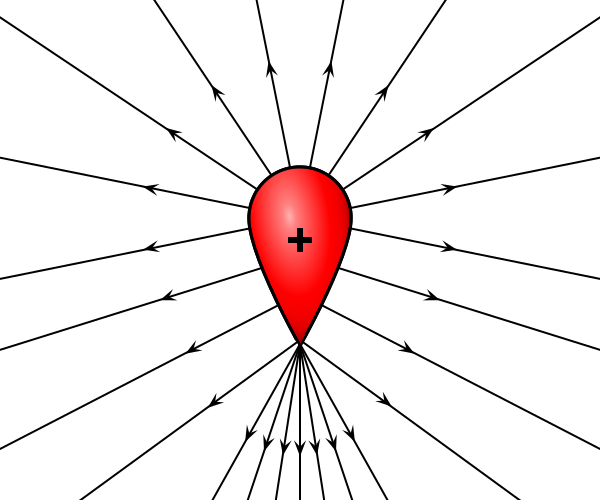
\includegraphics[width=4cm]{Bilder/electric-peak-field-static.pdf}}
\hspace{0.6cm}
\raisebox{-0.5\height}{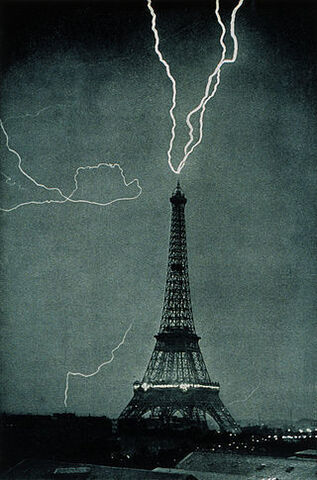
\includegraphics[width=4.2cm]{Bilder/lightning-striking-the-eiffel-tower-static.jpg}}
\end{center}
\end{hinweisbox}
\end{theoriebox}

\needspace{6cm}
\begin{questions}
\begin{taskbox}
\question[3] Erklären Sie in eigenen Worten und in ganzen Sätzen, wie aus
der Ladungstrennung in der Gewitterwolke ein Blitz entsteht. Gehen Sie dabei
auf die Reibungselektrizität, die influenzierte Ladung am Boden und die
kritische Feldstärke ein.
\begin{answerbox}
\vspace{2.4cm}
\end{answerbox}
\begin{solution}
Reibung zwischen Eiskristallen und Wassertröpfchen beim Auf- und Absteigen
in der Wolke trennt die Ladungen: oben positiv, unten negativ. Das Feld der
negativ geladenen Wolkenunterseite influenziert am Boden darunter positive
Ladung, die Erde wirkt also wie der positive Pol. Übersteigt das Feld
zwischen Wolke und Boden die kritische Feldstärke, gleichen sich die
Ladungen schlagartig aus: der Blitz.
\end{solution}
\end{taskbox}
\end{questions}

\textbf{Experiment: Elektroskop im Faradayschen Käfig}

\Bild{6.5cm}{Bilder/Tesla_Spule.JPG}

So eindrücklich funktioniert das Prinzip des Faradayschen Käfigs auch im
Grossen: Die Person im Bild steht in einem Gitterkäfig, während eine
Teslaspule meterlange Blitze auf sie zielt, und bleibt dabei unverletzt.
Genau dieses Prinzip untersuchen Sie jetzt im Kleinen.

Ein \textbf{\emph{Elektroskop}} zeigt elektrische Ladung an: Fliessen
Elektronen in den Metallstab, tragen Stab und Zeiger dieselbe Ladung und
stossen sich gegenseitig ab, der Zeiger schlägt aus.

\Bild{7.5cm}{Bilder/Elektroskop.pdf}

{\sloppy
Beobachten Sie das folgende Experiment: Ein Elektroskop steht innerhalb
eines Gitterkäfigs (\textbf{\emph{Faradayscher Käfig}}). Ein geladener Stab
wird von aussen angenähert.
\par}

\needspace{4cm}
\begin{questions}
\begin{taskbox}
\question[1] Notieren Sie Ihre Beobachtung.
\begin{answerbox}
\vspace{0.9cm}
\end{answerbox}
\begin{solution}
Das Elektroskop schlägt nicht aus, obwohl sich der geladene Stab dem Käfig
nähert.
\end{solution}
\end{taskbox}
\end{questions}

\needspace{10cm}
\begin{questions}
\begin{groupbox}[Gruppenarbeit: Erklären Sie die Beobachtung]
\question[6] Vervollständigen Sie zu zweit oder zu dritt die folgende
Skizze (zeichnen Sie ein, was mit der Ladungsverteilung, der Influenz und
dem elektrischen Feld im und um den Käfig passiert) und schreiben Sie dazu
einen kurzen Text, der erklärt, weshalb das Elektroskop im Käfiginneren
nicht ausschlägt. Verwenden Sie dabei alle drei Begriffe
\textbf{\emph{Ladungsverteilung}}, \textbf{\emph{Influenz}} und
\textbf{\emph{elektrisches Feld}}, und beschreiben Sie den Zusammenhang
zwischen ihnen, nicht nur die drei Begriffe einzeln.
\begin{answerbox}
\begin{center}
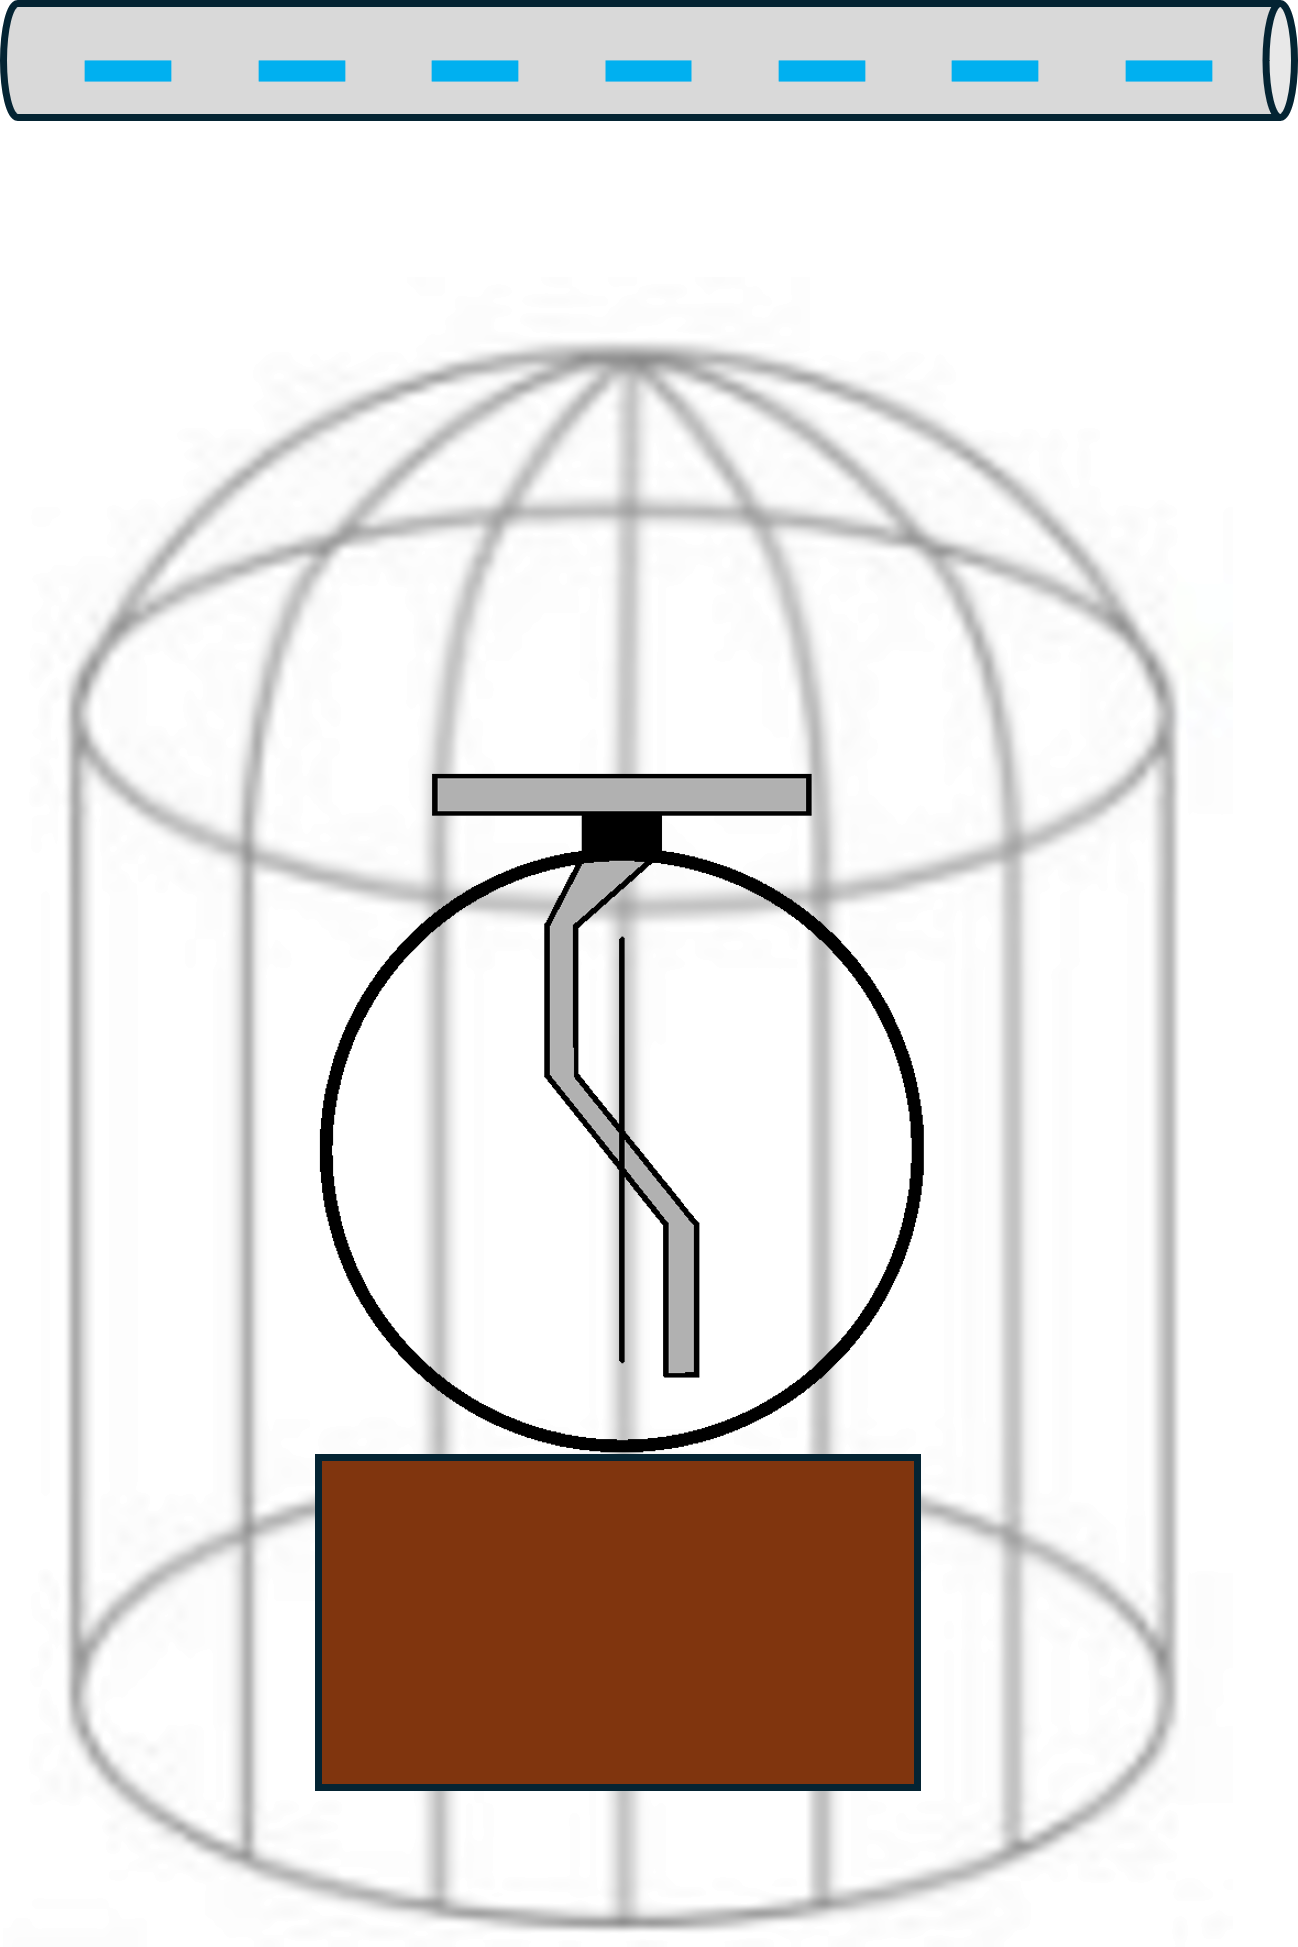
\includegraphics[width=5cm]{Bilder/Faraday_0.png}
\end{center}
\vspace{3cm}
\end{answerbox}
\begin{solution}
Das äussere Feld $\vec{E}_{\text{Stab}}$ des geladenen Stabs influenziert auf
dem Käfig eine Ladungsverteilung: Auf der dem Stab zugewandten Seite
sammeln sich ungleichnamige, auf der abgewandten Seite gleichnamige
Ladungen. Diese influenzierte Ladungsverteilung erzeugt selbst ein
elektrisches Feld $\vec{E}_{\text{FK}}$, das dem äusseren Feld im
Käfiginneren genau entgegengerichtet ist. Im Inneren heben sich die beiden
Felder deshalb exakt auf ($\vec{E}_{\text{Stab}}+\vec{E}_{\text{FK}}=0$),
ausserhalb dagegen nicht. Ein Leiter im elektrostatischen Gleichgewicht ist
also in seinem Inneren immer feldfrei. Das Elektroskop im Käfiginneren
spürt vom äusseren Feld nichts und schlägt deshalb nicht aus.

\begin{center}
\begin{tabular}{cc}
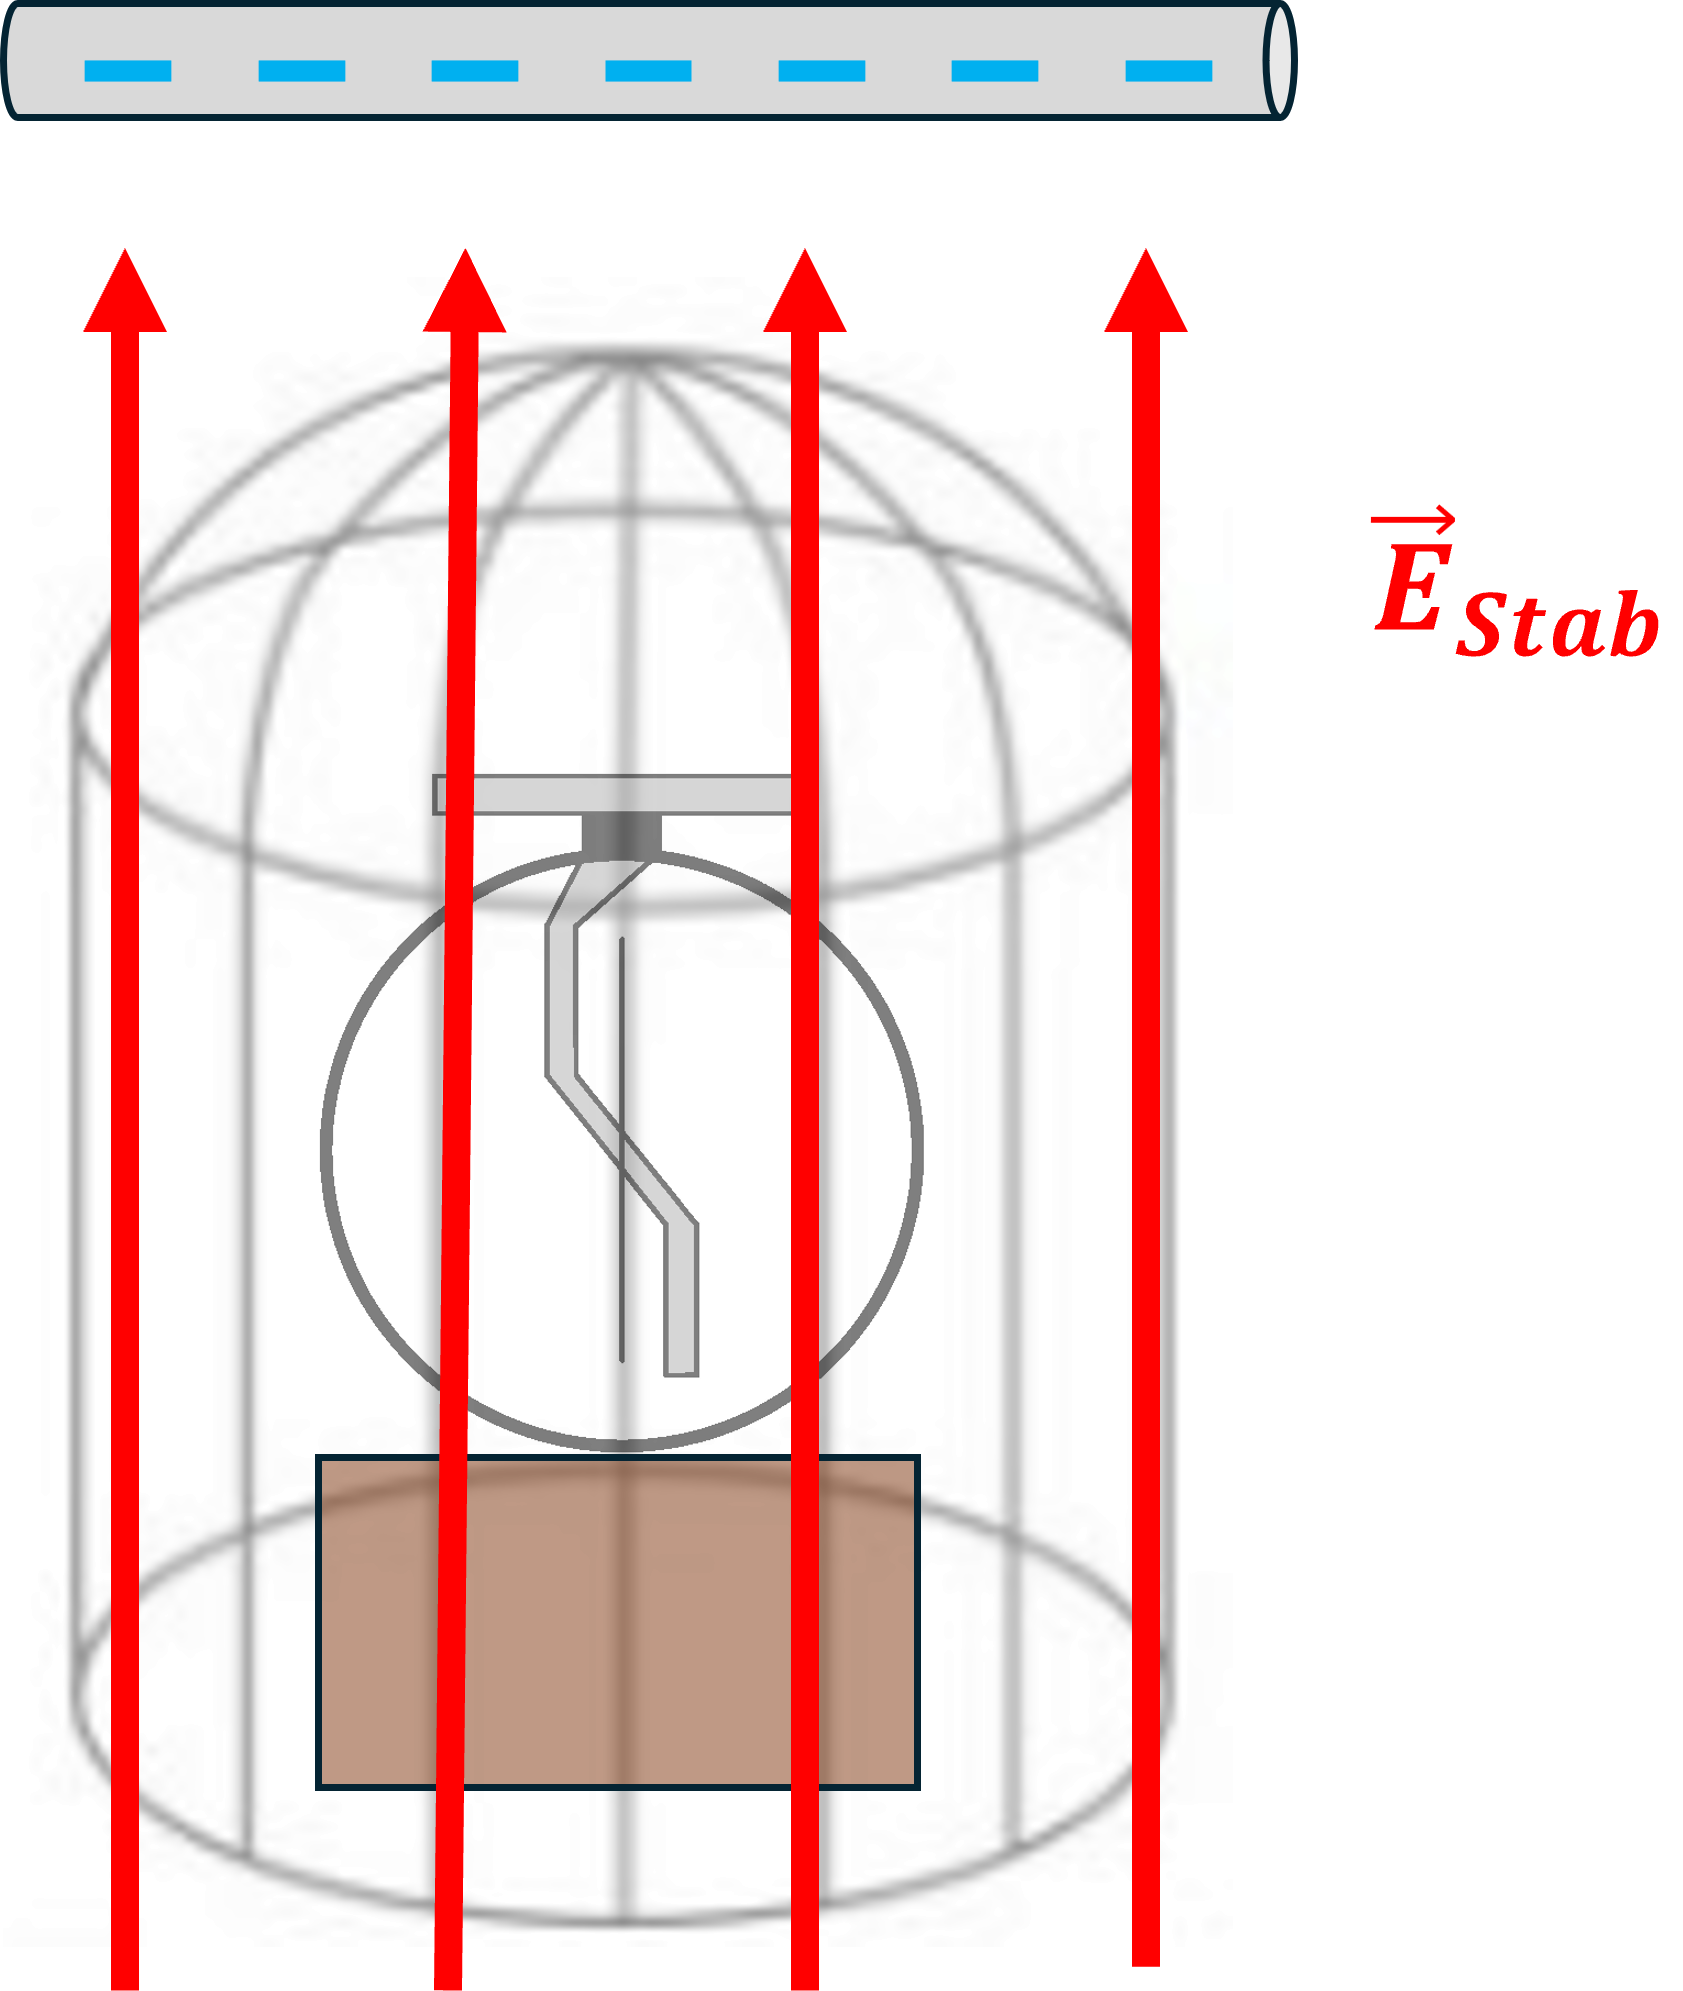
\includegraphics[width=3.9cm]{Bilder/Faraday_1.png} &
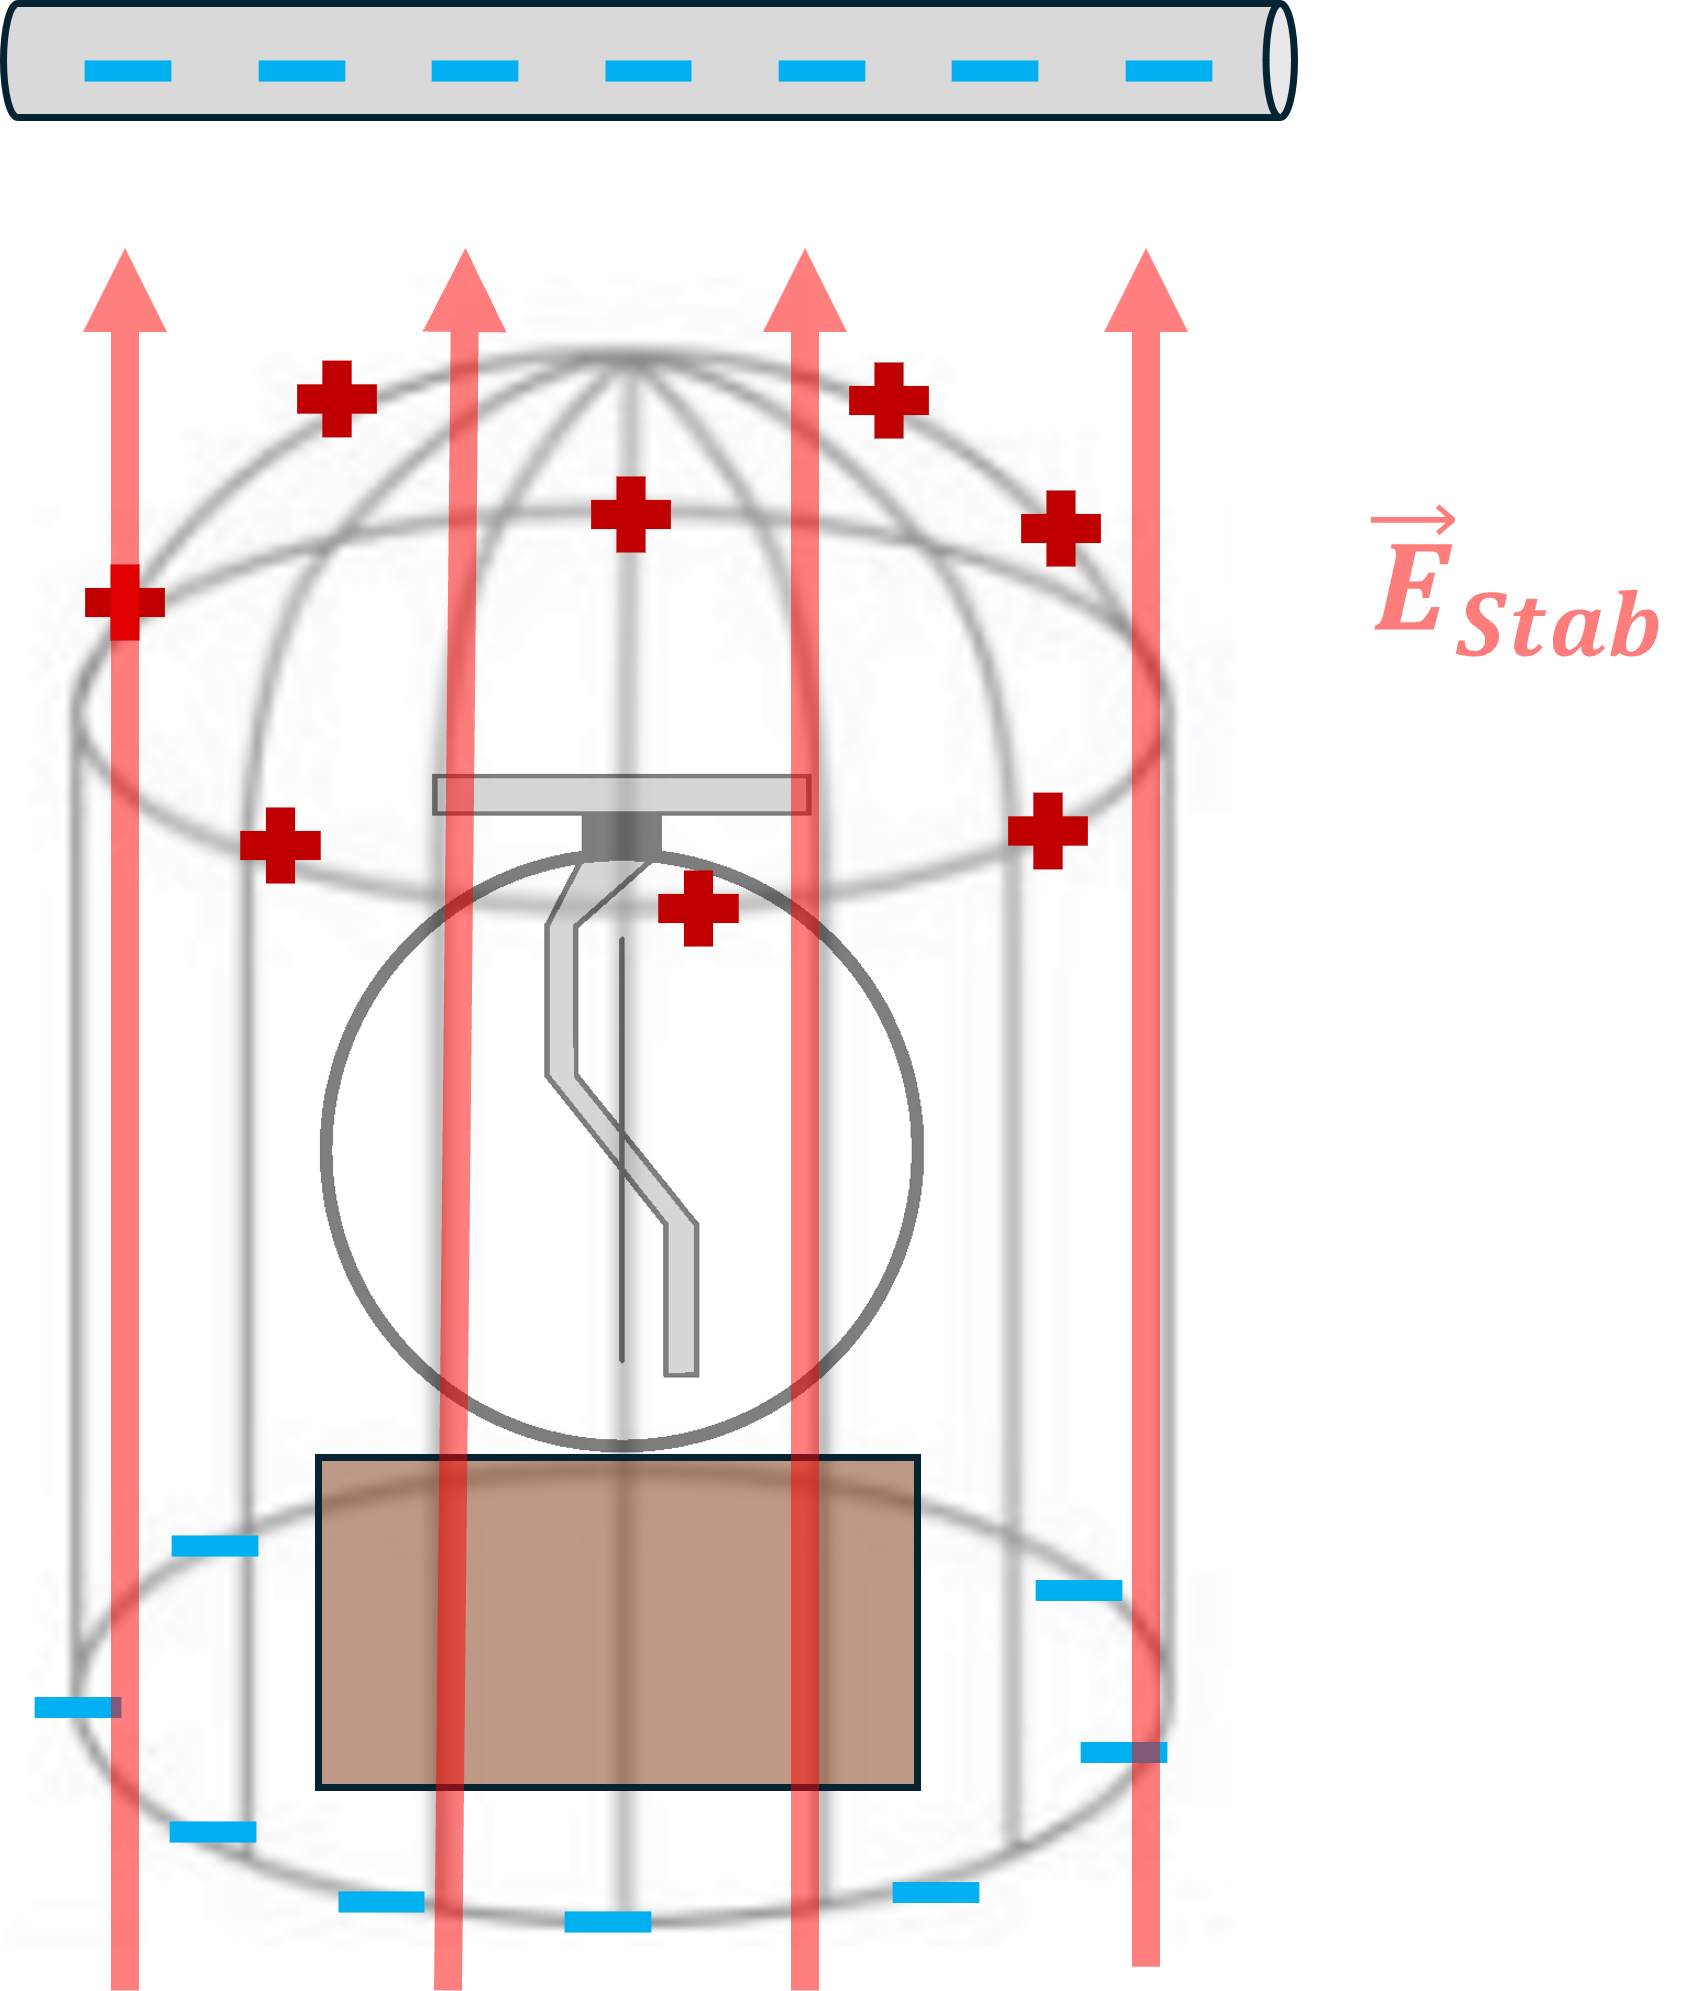
\includegraphics[width=3.9cm]{Bilder/Faraday_2.png} \\
(a) Feld $\vec{E}_{\text{Stab}}$ vor der Influenz &
(b) influenzierte Ladungsverteilung \\[0.8em]
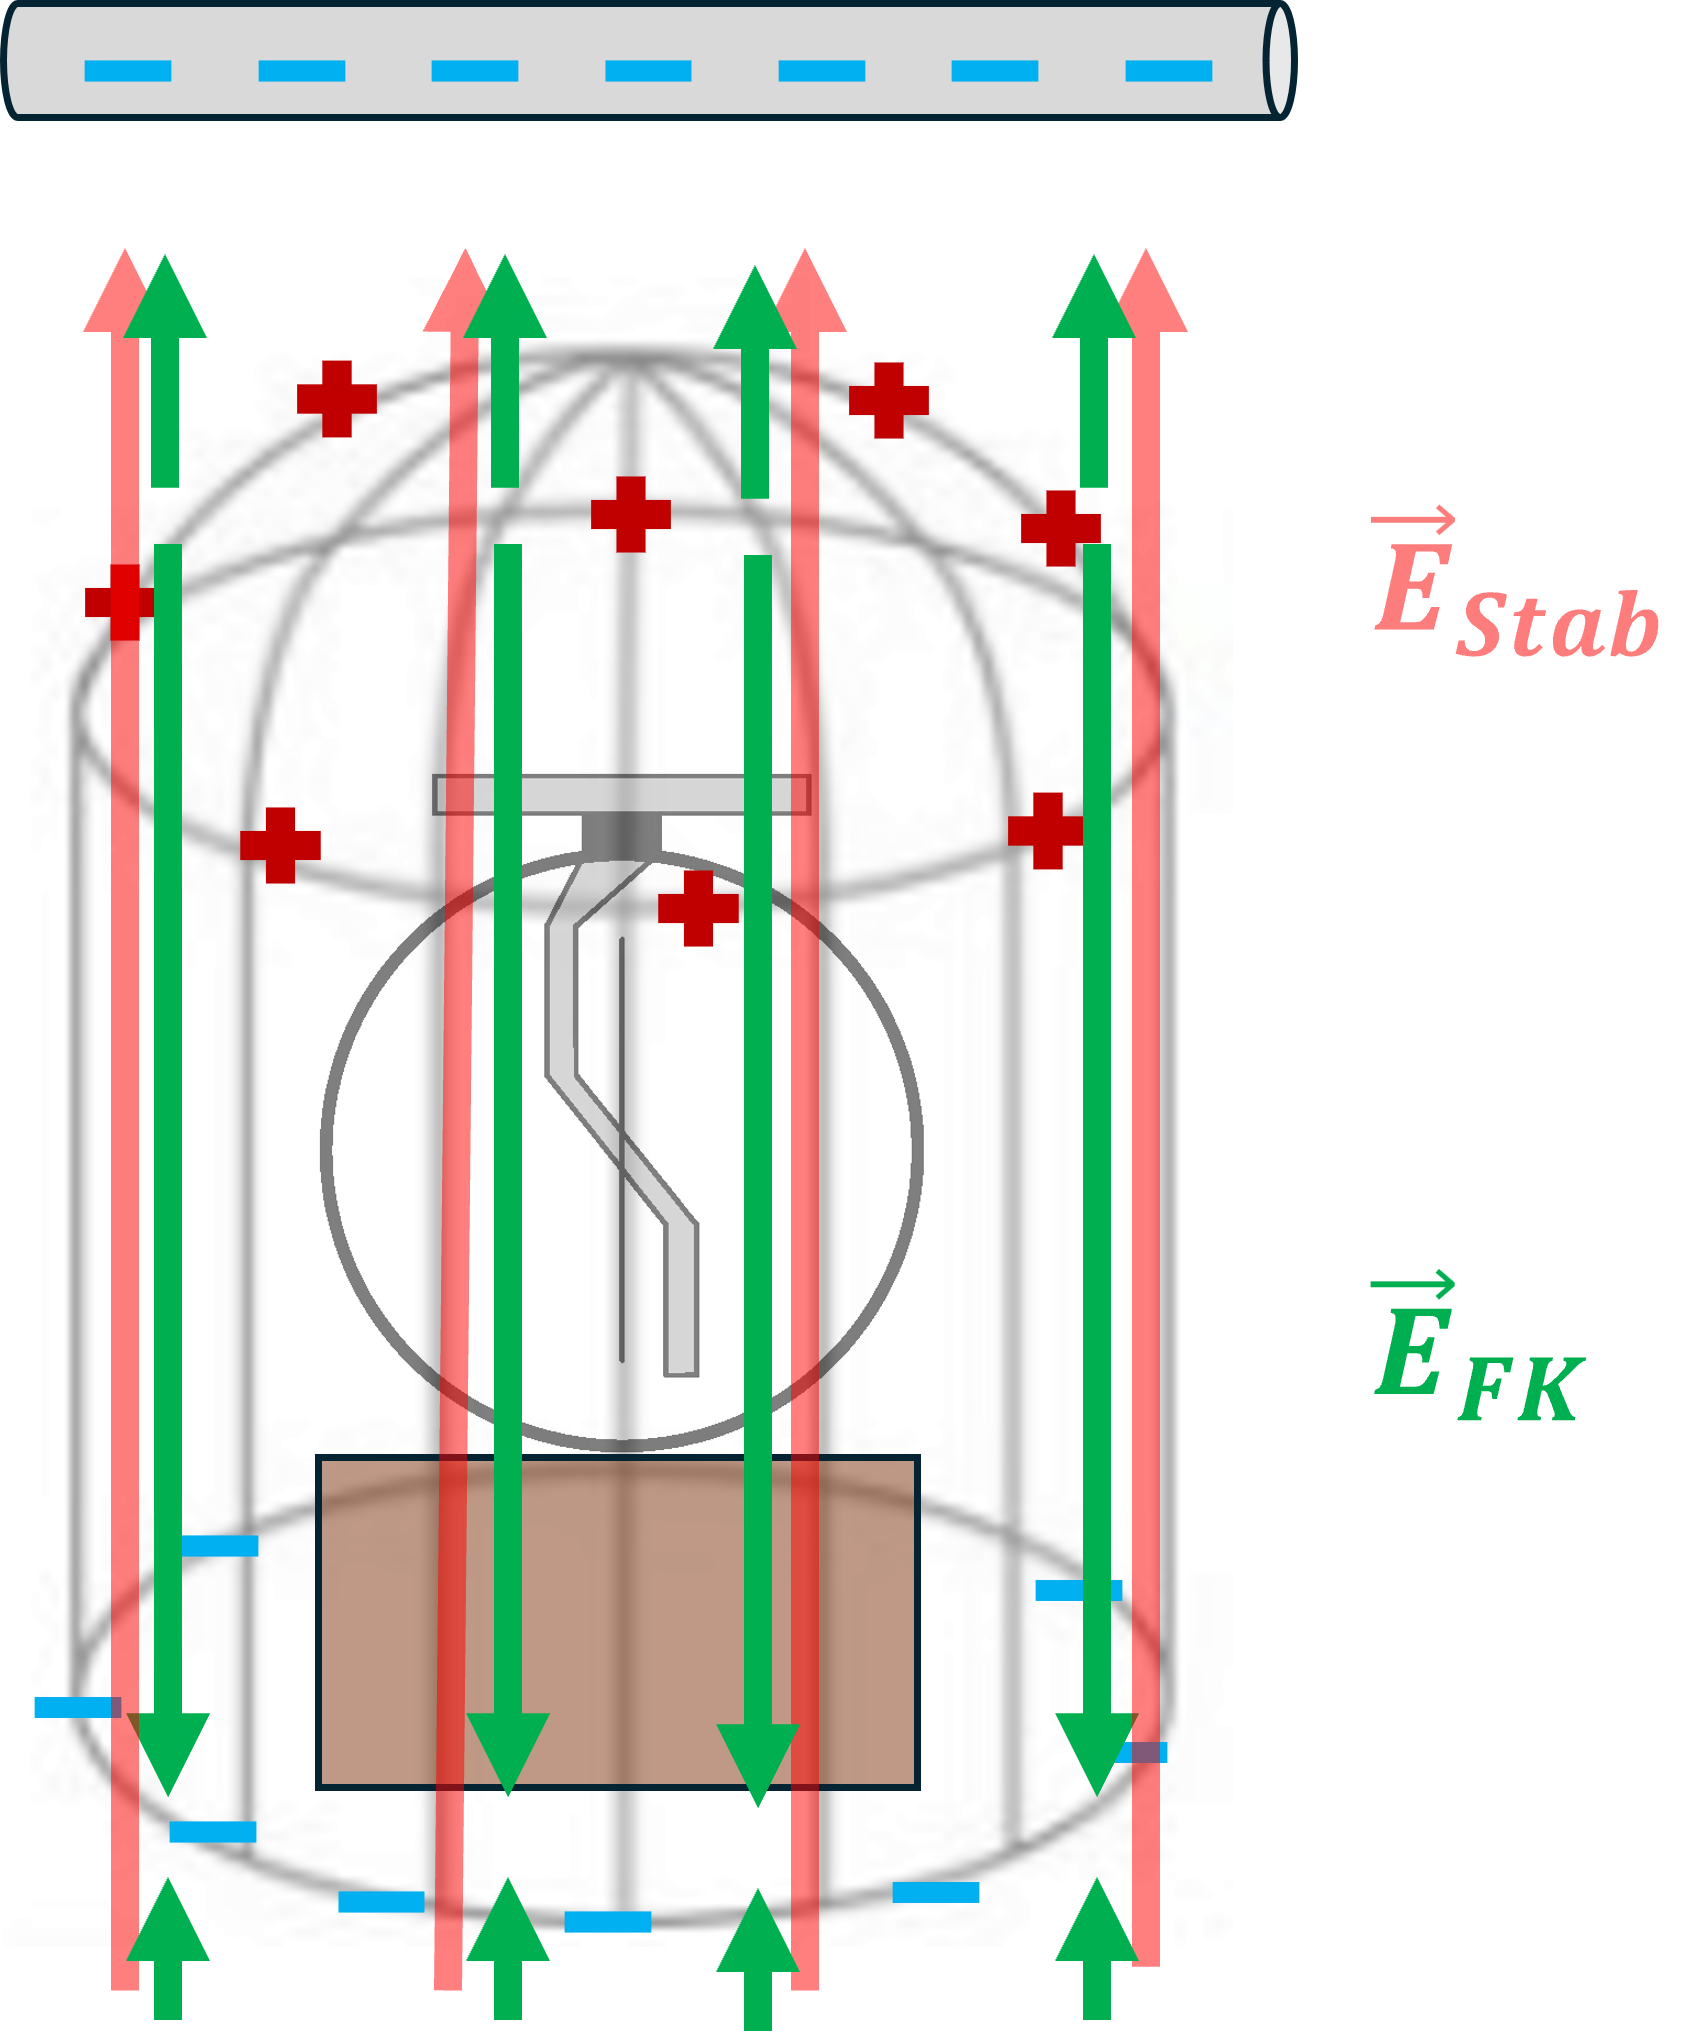
\includegraphics[width=3.9cm]{Bilder/Faraday_3.png} &
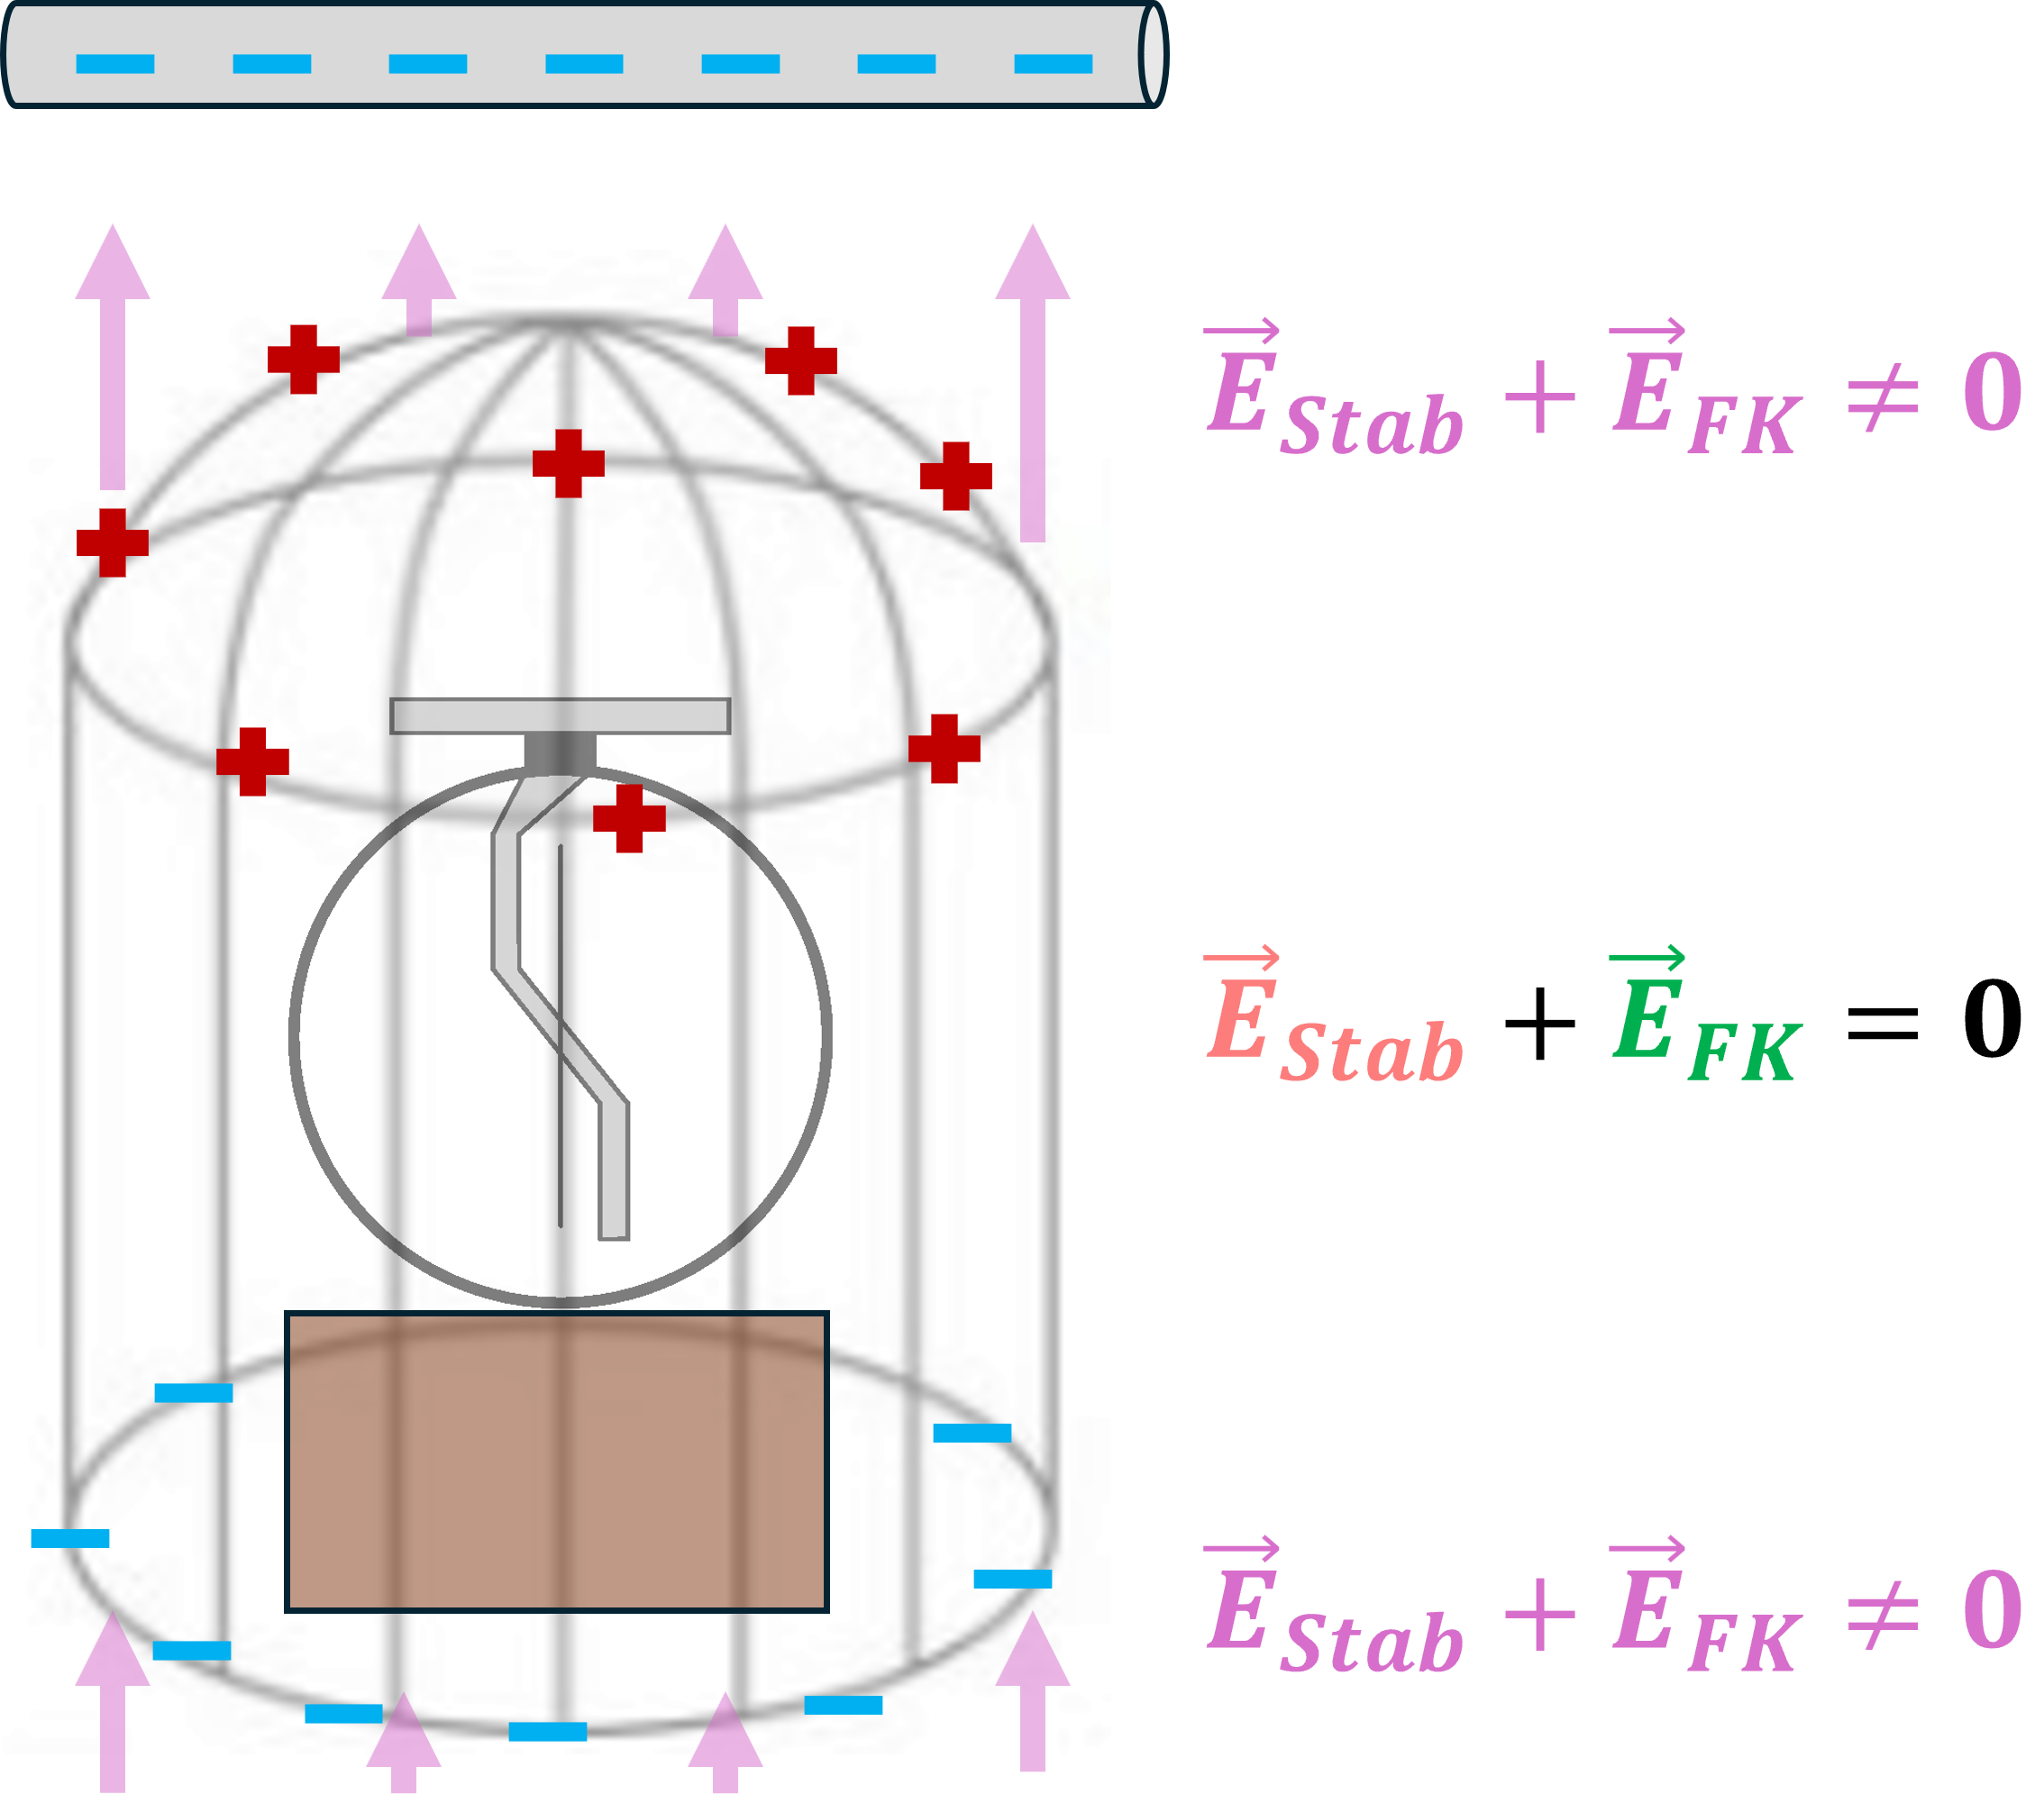
\includegraphics[width=3.9cm]{Bilder/Faraday_4.png} \\
(c) Gegenfeld $\vec{E}_{\text{FK}}$ der influenzierten Ladung &
(d) innen $0$, aussen $\vec{E}_{\text{Stab}}+\vec{E}_{\text{FK}}\neq 0$
\end{tabular}
\end{center}
\end{solution}
\end{groupbox}
\end{questions}

\needspace{12cm}
\begin{questions}
\begin{taskbox}[Übertragen: Auto und Haus als Faradayscher Käfig]
\question[3] Warum ist man in einem Auto oder Haus bei einem Gewitter
sicher? Was schützt wirklich, die Karosserie oder die Gummireifen?
Begründen Sie.

\begin{center}
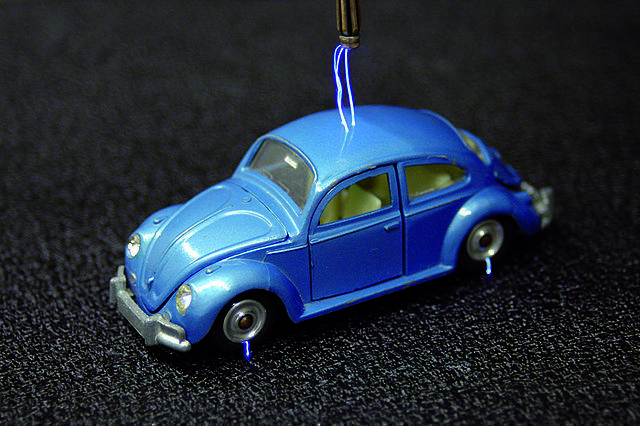
\includegraphics[width=5.4cm]{Bilder/faraday-cage-car-static.jpg}
\hspace{0.4cm}
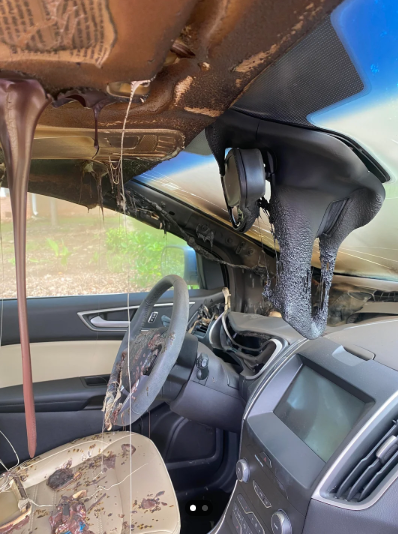
\includegraphics[width=3.6cm]{Bilder/auto_innenraum_blitzschlag.png}
\end{center}
\begin{answerbox}
\vspace{1.8cm}
\end{answerbox}
\begin{solution}
Die Metallkarosserie des Autos (bzw. das Metallgerüst/die Blitzschutzanlage
eines Hauses) wirkt als Faradayscher Käfig: Influenzierte Ladungen auf der
Karosserie kompensieren das äussere Feld im Innenraum. Die Gummireifen
spielen dabei keine Rolle. Der Blitz überspringt ohnehin die Lücke
zwischen Karosserie und Boden, statt durch die isolierenden Reifen zu
fliessen. Die Karosserie selbst kann dabei durchaus beschädigt werden
(Lack, Antenne, wie im rechten Bild oben zu sehen), der Innenraum bleibt
aber feldfrei und sicher.
\end{solution}
\end{taskbox}
\end{questions}

\needspace{9cm}
\begin{questions}
\begin{taskbox}[Diskussion: Schrittspannung]
\question[3] Betrachten Sie die folgende Darstellung der Schrittspannung
bei einem Blitzeinschlag.
\Bild{7cm}{Bilder/schrittspannung.jpg}
\begin{parts}
  \part[2] Besprechen Sie zu zweit: Warum ist es gefährlich, sich bei einem
  nahen Blitzeinschlag mit gespreizten Beinen hinzustellen oder gar
  wegzurennen?
  \begin{answerbox}
  \vspace{1.6cm}
  \end{answerbox}
  \begin{solution}
  Der Blitzstrom fliesst im Boden radial vom Einschlagpunkt weg, das
  Potenzial fällt also mit wachsendem Abstand vom Einschlagpunkt.
  Stehen die beiden Füsse unterschiedlich weit vom Einschlagpunkt entfernt
  (gespreizte Beine, grosse Schritte beim Rennen), liegt zwischen ihnen
  eine Potenzialdifferenz (die \textbf{\emph{Schrittspannung}}), die
  einen Strom durch den Körper treiben kann.
  \end{solution}

  \part[1] Welche Sicherheitsregel leiten Sie daraus ab?
  \begin{answerbox}
  \vspace{0.9cm}
  \end{answerbox}
  \begin{solution}
  Beine zusammenhalten und in die Hocke gehen, statt zu rennen oder breit
  zu stehen: So bleibt der Abstand zwischen den beiden Füssen und damit die
  Schrittspannung möglichst klein.
  \end{solution}
\end{parts}
\end{taskbox}
\end{questions}

\begin{beispielbox}[Auf einen Blick: sicher oder gefährlich?]
\Bild{9.5cm}{Bilder/Gewitter_Grafik_Jung.jpg}
\end{beispielbox}

\end{document}
